\documentclass[a4paper,10pt, notitlepage]{report}
\usepackage[utf8]{inputenc}
\usepackage{natbib}
\usepackage{amssymb}
\usepackage{amsmath}
\usepackage{amsthm}
\usepackage[shortlabels]{enumitem}
\usepackage{xurl}
\usepackage{hyperref}
% \usepackage[portuguese]{babel}

\usepackage{algorithm}
\usepackage{algpseudocode}
\usepackage{graphicx}

%%%%%%%%%%%%%%%%%%%%%%%%%%%%%%%%%%%%%%%%%%%%%%%%
% Proper definitions
%%%%%%%%%%%%%%%%%%%%%%%%%%%%%%%%%%%%%%%%%%%%%%%%
\newcommand{\R}{\mathbb{R}}
\newcommand{\Q}{\mathbb{Q}}
\newcommand{\Z}{\mathbb{Z}}
\newcommand{\N}{\mathbb{N}}
\newcommand{\tr}{\operatorname{tr}}
\newcommand{\var}{\operatorname{Var}}
\newcommand{\unif}{\operatorname{Unif}}
\newcommand{\ev}{\mathbb{E}}
\newcommand{\pr}{\mathbb{P}}


% Title Page
\title{Assignment 0: O Brother, How Far Art Thou?}
\author{Computational Statistics \\ Instructor: Luiz Max de Carvalho \\ Student: Lucas Machado Moschen}

\begin{document}
\maketitle

\textbf{Hand-in date: 06/10/2021.}

\section*{General guidance}
\begin{itemize}
 \item State and prove all non-trivial mathematical results necessary to substantiate your arguments;
 \item Do not forget to add appropriate scholarly references~\textit{at the end} of the document;
 \item Mathematical expressions also receive punctuation;
 \item Please hand in a single PDF file as your final main document.
 
 Code appendices are welcome,~\textit{in addition} to the main PDF document.
 \end{itemize}

\newpage

\section*{Background}

A large portion of the content of this course is concerned with computing high-dimensional integrals~\textit{via} simulation.
Today you will be introduced to a simple-looking problem with a complicated closed-form solution and one we can approach using simulation.

Suppose you have a disc $C_R$ of radius $R$. 
Take $p = (p_x, p_y)$ and $ q = (q_x, q_y) \in C_R$ two points in the disc.  
Consider the Euclidean distance between $p$  and $q$, $||p-q|| = \sqrt{(p_x-q_x)^2 + (p_y-q_y)^2} = |p-q|$.
\paragraph{Problem A:} What is the \textit{average} distance between pairs of points in $C_R$ if they are picked uniformly at random?

\section*{Questions}

\begin{enumerate}
 \item To start building intuition, let's solve a related but much simpler problem.
 Consider an interval $[0, s]$, with $s>0$ and take $x_1,x_2 \in [0, s]$~\textit{uniformly at random}.
 Show that the average distance between $x_1$ and $x_2$ is $s/3$.

 \begin{proof}[Solution]
    We want to calculate $\ev[|x_1 - x_2|]$ such that $x_1, x_2
    \overset{iid}{\sim} \unif(0,s)$. A long and default way to solve this problem is
    to introduce the random variable $Y = x_1 - x_2$, derive its density,
    and its absolute mean from the density. Let
    \begin{equation*}
        F_Y(y) = \pr(Y \le y) = \pr(x_1 \le y + x_2).
    \end{equation*}
    Suppose first that $y \ge 0$. Given
    $x_2$, 
    $$\pr(x_1 \le y + x_2|x_2) = \begin{cases}
        \dfrac{y + x_2}{s} &0 \le x_2 \le s - y \\
        1 &s - y < x_2 \le s.
    \end{cases}$$
    Therefore, 
    \begin{equation*}
        \begin{split}
            F_Y(y) &= \int_0^{s-y} \frac{y+x_2}{s^2} \, dx_2 + \int_{s-y}^s \frac{1}{s} \, dx_2  \\
            &= \frac{y(s-y) + 0.5(s-y)^2}{s^2} + \frac{y}{s} \\
            &= \frac{(s-y)(y + s)}{2s^2} + \frac{y}{s} = - \frac{y^2}{2s^2} + \frac{y}{s} + \frac{1}{2}.
        \end{split}
    \end{equation*}
    Now suppose $y < 0$. Then 
    $$\pr(x_1 \le y + x_2|x_2) = \begin{cases}
        \dfrac{y + x_2}{s} &-y \le x_2 \le s \\
        0 &0 \le x_2 < -y.
    \end{cases}$$
    Therefore, 
    \begin{equation*}
        \begin{split}
            F_Y(y) &= \int_{-y}^{s} \frac{y+x_2}{s^2} \, dx_2 \\
            &= \frac{ys + 0.5s^2}{s^2} - \frac{-y^2 + 0.5y^2}{s^2} \\
            &= \frac{y^2}{2s^2} + \frac{y}{s} + \frac{1}{2}.
        \end{split}
    \end{equation*}
    Deriving these expressions we get the density with respect to the Lebesgue
    measure, 
    \begin{equation*}
        f_Y(y) = \begin{cases}
            \dfrac{1}{s} - \dfrac{y}{s^2}, &\text{ if } 0 \le y \le s \\
            \dfrac{1}{s} + \dfrac{y}{s^2}, &\text{ if } -s \le y < 0. \\
        \end{cases}
    \end{equation*}
    Finally, 
    \begin{equation*}
        \begin{split}
            \ev[|x_1 - x_2|] = \ev[|Y|] &= \int_0^s \frac{y}{s} - \frac{y^2}{s^2} \, dy - \int_{-s}^0 \frac{y}{s} + \frac{y^2}{s^2} \, dy \\
            &= \frac{s^2}{2s} - \frac{s^3}{3s^2} + \frac{s^2}{2s} - \frac{s^3}{3s^2} \\
            &= \frac{s}{2} - \frac{s}{3} + \frac{s}{2} - \frac{s}{3} = \frac{s}{3},
        \end{split}
    \end{equation*}
    as we wished to prove. Now I give a more geometric approach. Consider
    $(x_1, x_2)$ uniformly distributed over $[0,1]^2$. Then, let $t \in [0,s]$, 
    $$
    \pr(|x_1 - x_2| > t) = \pr(x_1 > t + x_2) + \pr(x_2 > t + x_1),
    $$
    since they are disjoint events for $t \ge 0$. Note that the 
    first region is delimited by the straight lines $x_1 = t + x_2$, $x_1 = s$,
    and $x_2 = 0$, what gives a triangle with points $(t,0), (s, 0), $ and
    $(s,s-t)$
    with area $(s-t)^2/2$. The second region is delimited by the straight lines
    $x_2 = t + x_1$, $x_2 = s$, and $x_1 = 0$, what gives the triangle 
    $(0,t), (0,s)$ and $(s-t,s)$, with area $(s-t)^2/2$. We conclude that
    $$
    \pr(|x_1 - x_2| > t) = \frac{(s-t)^2}{s^2} \text{ if } t \in [0,s], 
    $$
    using the fact that the density of $(x_1, x_2)$ is $s^{-2}$. This implies that 
    $$
    \ev[|x_1 - x_2]] = \int_0^{+\infty} \frac{(s-t)^2}{s^2} 1_{\{t \le s\}} \, dt
    = -\frac{(s-t)^3}{3s^2}\bigg|_{0}^s = \frac{s}{3},
    $$
    a simpler prove. 
 \end{proof}

 \item Show that Problem A is equivalent to computing
 \begin{equation*}
    \frac{1}{\pi^2 R^4}\int_{0}^{R}\int_{0}^{R}\int_{0}^{2\pi}\int_{0}^{2\pi}\sqrt{r_1^2 + r_2^2 - 2r_1r_2\cos\phi(\theta_1, \theta_2)}r_1r_2\,d\theta_1\,d\theta_2\,dr_1\,dr_2,
   \end{equation*}
   where $\phi(\theta_1, \theta_2)$ is the central angle between $r_1$ and $r_2$.

   \begin{proof}[Solution]
       Let $p = (p_x, p_y)$ e $q = (q_x, q_y)$ points in the disc of radius $R$.  We are interested
       in the quantity
       $$\ev\left[\sqrt{(p_x - q_x)^2 + (p_y - q_y)^2}\right].$$ Transforming
       to polar coordinates, 
       $$
       p_x = r_1\cos(\theta_1), p_y = r_1\sin(\theta_1), q_x = r_2\cos(\theta_2), q_y = r_2\sin(\theta_2).
       $$
       And we have the following relation. 
        \begin{equation*}
            \begin{split}
                (p_x - q_x)^2 + (p_y - q_y)^2 &= r_1^2\cos(\theta_1)^2 + r_2^2\cos(\theta_1) - 2r_1r_2\cos(\theta_1)\cos(\theta_2) \\ 
                &+ r_1^2\sin(\theta_1)^2 + r_2^2\sin(\theta_1) - 2r_1r_2\sin(\theta_1)\cos(\theta_2) \\ 
                &= r_1^2 + r_2^2 -2r_1r_2\cos(\theta_1 - \theta_2),
            \end{split}
        \end{equation*}
        using the appropriate trigonometric relations. Let $p = (p_x, p_y)$ e $q = (q_x, q_y)$ pontos aleatórios com
        distribuição uniforme no disco de raio $R$. Consider a system of
        coordinates in which the origin is the center of the disc. We know that the density
        of the distribution of $p$ with respect to the Lebesgue measure is 
        $$
        f(p) = \frac{1}{\pi R^2}1_{\{||p|| \le R\}}.
        $$
        The same for $q$. Now we want to transform this distribution to polar
        coordinates, in which $\theta_1 \in [0,2\pi]$ and $r_1 \in [0,R]$. The
        Jacobian of the inverse transformation is given by 
        $$
        \begin{bmatrix}
            \cos(\theta_1) & -r_1\sin(\theta_1) \\
            \sin(\theta_1) & r_1\cos(\theta_1),
        \end{bmatrix}
        $$
        in which the absolute value of the determinant is $r_1$. By the Change of Variables in probability density function, 
        $$
        g_1(r_1, \cos(\theta_1)) = \frac{1}{\pi R^2}r_1. 
        $$
        Notice that the same happens with $(r_2, \cos(\theta_2))$ with 
        $$
        g_2(r_2, \cos(\theta_2)) = \frac{1}{\pi R^2}r_2. 
        $$
        By the Law of the unconscious statistician and the transformations
        made above, $\ev\left[\sqrt{(p_x - q_x)^2 + (p_y - q_y)^2}\right] = $
        $$
        \int_{A_1} \int_{A_2} \sqrt{r_1^2 + r_2^2 -2r_1r_2\cos(\theta_1 - \theta_2)}g_1(r_1, \theta_1)g_2(r_2, \theta_2) \, dA_2 \, dA_1, 
        $$
        such that $A_i = [0,R] \times [0,2\pi]$, for $i=1,2$. Given that the
        integrand is non negative, by Tonelli's
        Theorem \cite[]{rosenthal2006first}, the integral is 
        $$
        \frac{1}{\pi^2 R^4}\int_{0}^{R}\int_{0}^{R}\int_{0}^{2\pi}\int_{0}^{2\pi}\sqrt{r_1^2 + r_2^2 - 2r_1r_2\cos(\theta_1 -\theta_2)}r_1r_2\,d\theta_1\,d\theta_2\,dr_1\,dr_2.
        $$
   \end{proof}

 \item Compute $I$ in closed-form.
 
 \begin{proof}[Solution]
    Following the hint, we shall use the Crofton's mean value theorem.
    However, instead of only using it, we will derive it from the beginning
    for this particular case to gain intuition. Let $I(R)$ be the integral
    above as a function of $R$. Consider the mapping $x \mapsto Rx$ from the
    unit circle to the $R$-circle. It is a linear function, so it is
    bijective. Besides that, 
    $$
    ||Rx - Ry|| = R||x-y||, 
    $$
    for all $x,y$ in the unit circle. This implies that 
    $$I(R) = RI(1) \text{ and } I'(R) = I(1).$$ 
    Let $\epsilon > 0$ and define $A^{\circ}$ the region delimited by the circle
    of radius $R - \epsilon$, $A$ de region delimited by the circle of radius
    $R$, and $\partial A = A / A^{\circ}$. By the Law of Total Expectation, 
    \begin{equation}
        \label{eq:law-total-expectation}
        \begin{split}
            I(R) = I(R - \epsilon)\pr(p,q \in A^{\circ}) &+ 2J(A^{\circ}, \partial A)\pr(p \in A^{\circ}, q \in \partial A) \\ 
            &+ K(\partial A)\pr(p, q \in \partial A),
        \end{split}
    \end{equation}
    such that $J(A^{\circ}, \partial A)$ is the expected distance between a
    point in the inner circle and the other in the outer circle, and
    $K(\partial A)$ the expected distance between points in the outer circle.
    We will take $\epsilon$ infinitely small afterwards. For that, note the
    following relations, 
    \begin{align*}
        \pr(p,q \in A^{\circ}) &= \left(\frac{\pi(R-\epsilon)^2}{\pi R^2}\right)^2 \\
        &= \frac{(R-\epsilon)^4}{R^4} = \sum_{k=0}^4 \binom{4}{k} (-1)^k R^{-k}\epsilon^{k} \\ 
        &= 1 - \frac{4\epsilon}{R} + o(\epsilon),  
    \end{align*}
    in which $o(\cdot)$ is the little o-notation, 
    \begin{align*}
        \pr(p \in A^{\circ}, q \in \partial A) &= \frac{(R-\epsilon)^2}{R^2}\left(1 - \frac{(R-\epsilon)^2}{R^2}\right) \\
        &= \frac{(R^2 -2R\epsilon + \epsilon^2)(2R\epsilon - \epsilon^2)}{R^4} \\ 
        &= \frac{2\epsilon}{R} + o(\epsilon),
    \end{align*}
    and 
    \begin{align*}
        \pr(p,q \in \partial A) &= \left(1 - \frac{(R-\epsilon)^2}{R^2}\right)^2 \\
        &= \frac{(2R\epsilon - \epsilon^2)^2}{R^4} \\ 
        &=o(\epsilon).
    \end{align*}
    The formula given by \eqref{eq:law-total-expectation} can be rewritten as 
    \begin{equation*}
        I(R) = I(R - \epsilon)\left(1 - \frac{4\epsilon}{R} + o(\epsilon)\right) + J(A^{\circ}, \partial A)\left(\frac{4\epsilon}{R} + o(\epsilon)\right) + K(\partial A)o(\epsilon),
    \end{equation*} 
    then 
    $$
    I(1) = I'(R) = \lim_{\epsilon \to 0} \frac{I(R) - I(R-\epsilon)}{\epsilon} = -\frac{4}{R}I(R) + \frac{4}{R}J(A,A),
    $$
    using the fact that $I$ and $J$ are continuos function (they are integrals
    of continuos functions). The above formula is what is known for Crofton's
    formula \cite[p. 100]{solomon1978geometric}. 
    
    It remais to calculate the expected distance between a point in
    the boundary of the circle and a point in the interior, $J(A,A)$. Without
    loss of generality, suppose that $p$ is in the border and $q$ in the
    interior of the circle. By its symmetry, and using the fact that distances are invariant to
    translations, we place $p$ at the origin and the center of the circle the $x$-axis. That said, the distance between
    the points is only $r_2$. Then, 
    $$
    J(A,A) = \frac{1}{\pi R^2}\int_A r_2 dA. 
    $$
    In polar coordinates, $q$ can be defined by $(r_2, \theta_2)$. Notice that
    $$-\pi/2 \le \theta_2 \le \pi/2.$$
    Besides that, let $c = \sup_{q \in \text{circle}}r_2$, then $c$ is the distance between $p$ and
    another point in the boundary of the circle. This distance can be
    calculated using the Law of Cosines for the triangle delimited by these
    points and the center. Then, $c = \sqrt{R^2 + R^2 - 2R^2\cos(\pi -
    2\theta)} = R\sqrt{2(1 + \cos(2\theta))}$. Since $\cos(2x) = \cos(x)^2 -
    \sin(x)^2 = 2\cos(x)^2 - 1$, we have that 
    $c = R\sqrt{4\cos(\theta)^2} = 2R\cos(\theta)$, that is, 
    $$
    0 \le r_2 \le 2R\cos(\theta),
    $$
    and (applying the Jacobian again), 
    \begin{align*}
        J(A,A) &= \frac{1}{\pi R^2} \int_{-\pi/2}^{\pi/2} \int_0^{2R\cos(\theta)} r_2^2 \, dr_2 \, d\theta_2 \\
        &= \frac{1}{\pi R^2} \int_{-\pi/2}^{\pi/2} \frac{8R^3}{3}\cos(\theta_2)^3 \, d\theta_2 \\
        &= \frac{1}{\pi R^2} \int_{-\pi/2}^{\pi/2} \frac{8R^3}{3}(1 - \sin(\theta_2)^2)\cos(\theta_2) \, d\theta_2 \\
        &= \frac{8R}{3\pi} \int_{-1}^{1} (1 - u^2) \, du \\
        &= \frac{32R}{9\pi}. \\
    \end{align*}
    Finally, 
    $$
    I(1) = -\frac{4}{R}I(R) + \frac{4}{R}\frac{32R}{9\pi} = -4I(1) + \frac{128}{9\pi} \implies I(1) = \frac{128}{45\pi},
    $$
    and 
    \begin{equation}
        \label{eq:closed-form}
        I(R) = \frac{128}{45\pi}R.
    \end{equation}
    We conclude that $I$ has a closed form given by \eqref{eq:closed-form}.
\end{proof}



 \item Propose a simulation algorithm to approximate $I$.
 Provide point and interval estimates and give theoretical guarantees about
 them (consistency, coverage, etc).
 
\begin{proof}[Solution]

 Consider the following transformation, 
 $$
 p_x = \sqrt{r_1}\cos(\theta_1), p_y = \sqrt{r_1}\sin(\theta_1), q_x = \sqrt{r_2}\cos(\theta_2), q_y = \sqrt{r_2}\sin(\theta_2).
 $$
 The Jacobian of this transformation is 
 $$
 \begin{bmatrix}
    \frac{1}{2\sqrt{r_1}}\cos(\theta_1) & -\sqrt{r_1}\sin(\theta_1) \\
    \frac{1}{2\sqrt{r_1}}\sin(\theta_1) & \sqrt{r_1}\cos(\theta_1),
\end{bmatrix}
 $$
 whose determinant is $1/2$, then the distribution is 
 $$
 g(r_1, \theta_1) = \frac{1}{2\pi R^2}1_{[0,R^2] \times [0,2\pi]}, 
 $$
 what is the uniform distribution in $[0,R^2] \times [0,2\pi]$. Then the
 algorithm can be as follows

 \begin{algorithm}
    \caption{Simulation for problem A}\label{alg:problem-A}
    \begin{algorithmic}
    \Require $R > 0$, n\_samples positive integer
    \State $r_1 \gets \operatorname{Uniform}$(lower = 0, upper = $1$, length = n\_samples)
    \State $r_2 \gets \operatorname{Uniform}$(lower = 0, upper = $1$, length = n\_samples)
    \State $\theta_1 \gets \operatorname{Uniform}$(lower = 0, upper = $1$,
    length = n\_samples)
    \State $\theta_2 \gets \operatorname{Uniform}$(lower = 0, upper = $1$,
    length = n\_samples)
    
    \State $\text{dist} \gets \sqrt{r_1^2 + r_2^2 - 2r_1r_2\cos(2\pi(\theta_1 -
    \theta_2))}$ 

    \State mean\_dist $\gets R\cdot \operatorname{mean}$(dist)

    \end{algorithmic}
\end{algorithm}

We want to evaluate the following integral, which is equivalent to $I$, as
already mentioned previously

$$
\frac{1}{4\pi^2 R^4}\int_{0}^{R^2}\int_{0}^{R^2}\int_{0}^{2\pi}\int_{0}^{2\pi}\sqrt{r_1 + r_2 - 2\sqrt{r_1r_2}\cos(\theta_1 -\theta_2)}\,d\theta_1\,d\theta_2\,dr_1\,dr_2.
$$

We use the following Monte Carlo simulation, let 
$$
\{r_1^{(n)}\}_{1 \le n \le N}, \{r_2^{(n)}\}_{1 \le n \le N}
, \{\theta_1^{(n)}\}_{1 \le n \le N}
, \{\theta_2^{(n)}\}_{1 \le n \le N} \overset{iid}{\sim} \operatorname{Unif}(0,1)
$$
and 
$$
I^{MC}_N = \frac{R}{N}\sum_{k=1}^N \sqrt{r_1^{(k)} + r_2^{(k)} - 2\sqrt{r_1^{(k)}r_2^{(k)}} \cos(2\pi(\theta_1^{(k)} -\theta_2^{(k)}))}.
$$

By the Strong Law of Large Numbers, $I_N^{MC}$ converges almost surely to $I$.
Now we want to calculate the variance of the desired quantity. The second
moment is given by 

\begin{align*}
    &\frac{1}{\
    4\pi^2 R^4}\int_{0}^{R^2}\int_{0}^{R^2}\int_{0}^{2\pi}\int_{0}^{2\pi}r_1 + r_2 - 2\sqrt{r_1r_2}\cos(\theta_1 -\theta_2)
    \,d\theta_1\,d\theta_2\,dr_1\,dr_2. \\
    &= \frac{1}{4\pi^2 R^4}\int_{0}^{R^2}\int_{0}^{R^2}\int_{0}^{2\pi} 2\pi(r_1+r_2) \,d\theta_2\,dr_1\,dr_2 \\ 
    &= \frac{1}{4\pi^2 R^4}\int_{0}^{R^2}\int_{0}^{R^2} 4\pi^2(r_1+r_2) \,dr_1\,dr_2 \\
    &= \frac{1}{R^4}\int_{0}^{R^2} \frac{1}{2}R^4 + R^2r_2 \,dr_2 = \frac{1}{R^4}(\frac{1}{2}R^6 + \frac{1}{2}R^6) = R^2,
\end{align*}
therefore 
$$
V = \var\left[\sqrt{(p_x - q_x)^2 + (p_y - q_y)^2}\right] = \left(1 - \left(\frac{128}{45\pi}\right)^2\right)R^2,
$$

which can also be estimated by Monte Carlo Simulation. This expression tell us
that the variance increases quadratically with $R$. The rate of convergence of
this estimator is $O(n^{-1/2})$, but it also depends on $R$, as already
mentioned. In order to provide interval estimates, by the Central Limit
Theorem, 
$$\sqrt{N}(I_N^{MC} - I) \overset{d}{\to} \operatorname{Normal}(0, V).$$
Supposing the standard deviation known, the confidence interval for $I$ is
$$I_N^{MC} \pm \Phi^{-1}\left(1 - \frac{\alpha}{2}\right)\frac{\sqrt{V}}{\sqrt{N}},$$
such that $\alpha$ is the level (commonly $\alpha = 0.05$) and $\Phi$ is the
normal cumulative distribution. When it is unknown, 
$$I_N^{MC} \pm T_{N-1}^{-1}\left(1 - \frac{\alpha}{2}\right)\frac{\sigma
'}{\sqrt{N}},$$
with $T_{n-1}$ being the cumulative distribution of t-Student with $n-1$
degrees of freedom and $\sigma '^2$ which is the unbiased Monte Carlo estimator
for $V$.

In Table \ref{tab:simulations}, we provide some information about the simulations with $R
= 5$. The confidence intervals converge to the same value with $N = 100$, which
shows the Monte Carlo convergence for the variance. The point estimates also
approximate to the true value 4.527. Figure \ref{fig:simulations} presents
these results graphically. As we have already mentioned, the
variance is affected by $R$. In that sense, Figure \ref{fig:simulations-r}
presents how the point estimates are affected by it. We put
$10000$ simulations and we conclude that there is an increase of the variance
of the error, but the relative error no. Therefore, if the precision need to
be constant for different $R$ values, more simulations are needed. 

The code is available in \url{https://github.com/lucasmoschen/Computational_Statistics/blob/master/assignments/warmup_assignment/simulation.py}.

\begin{table}[ht]
    \centering
    \begin{tabular}{|c|c|c|c|c|}
    \hline
    \textbf{$N$} & \textbf{Time(s)} & \textbf{Point estimate} & \textbf{95 CI (known V)} & \textbf{95 CI} \\ \hline
    $10^1$          & 0.0001161             & 4.9346                  & (3.62, 6.25)             & (3.59, 6.28)               \\ \hline
    $10^2$          & 0.0001843             & 4.6448                  & (4.23, 5.06)             & (4.24, 5.04)               \\ \hline
    $10^3$         & 0.0002418             & 4.5683                  & (4.36, 4.62)             & (4.36, 4.62)               \\ \hline
    $10^4$        & 0.001179              & 4.5466                  & (4.51, 4.59)             & (4.51, 4.59)               \\ \hline
    $10^5$       & 0.01124               & 4.5247                  & (4.51, 4.54)             & (4.51, 4.54)               \\ \hline
    $10^6$      & 0.1318                & 4.5264                  & (4.52, 4.53)             & (4.52, 4.53)               \\ \hline
    \end{tabular}
\caption{Simulations results for some values of $N$.}
\label{tab:simulations}
\end{table}

\begin{figure}[ht]
    \centering
    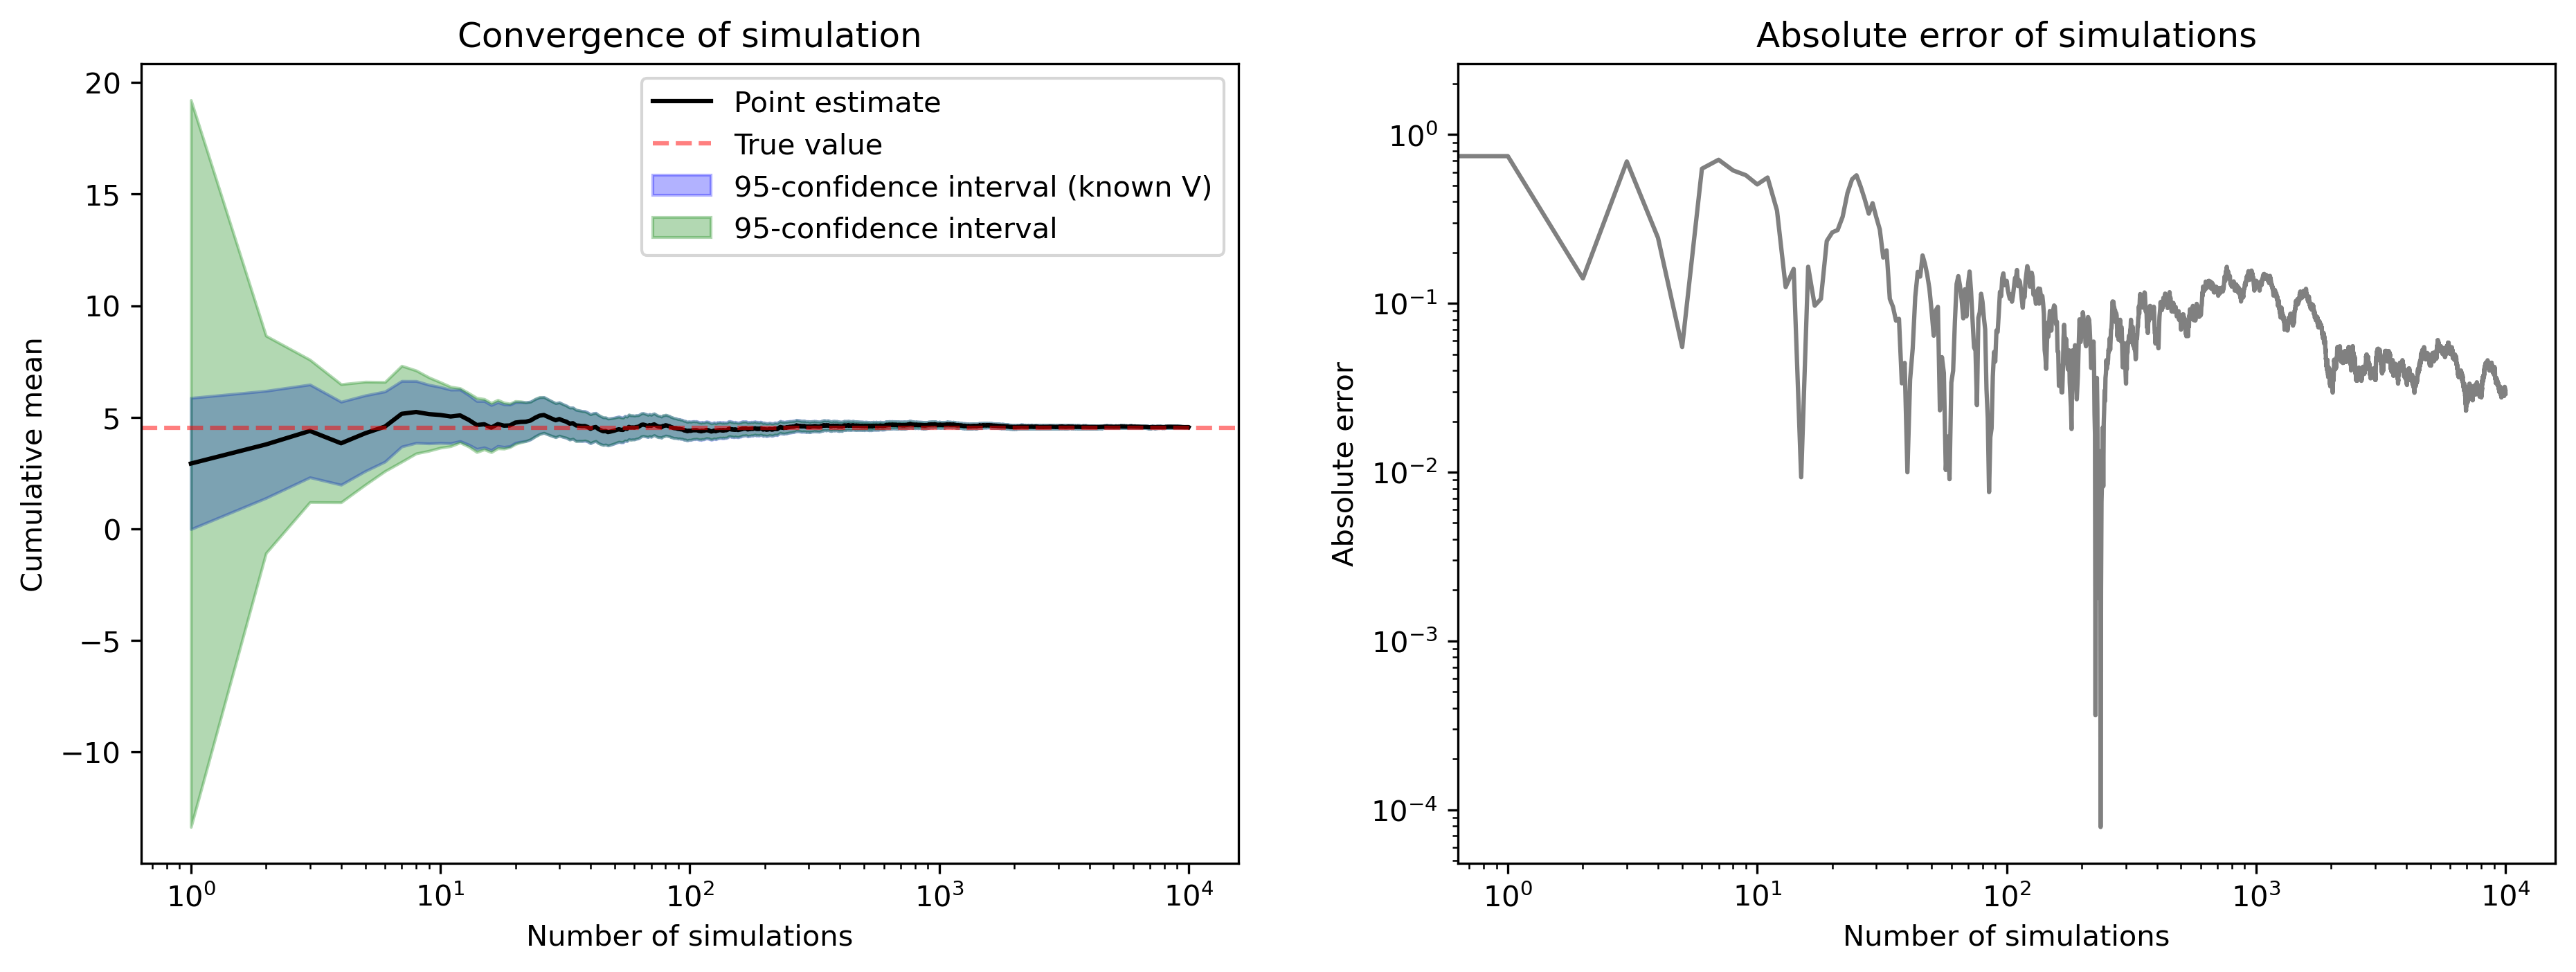
\includegraphics[width=\textwidth]{figure_simulation.png}
    \caption{Convergence figure and absolute error for different values of $N$.}
    \label{fig:simulations}
\end{figure}

\begin{figure}[ht]
    \centering
    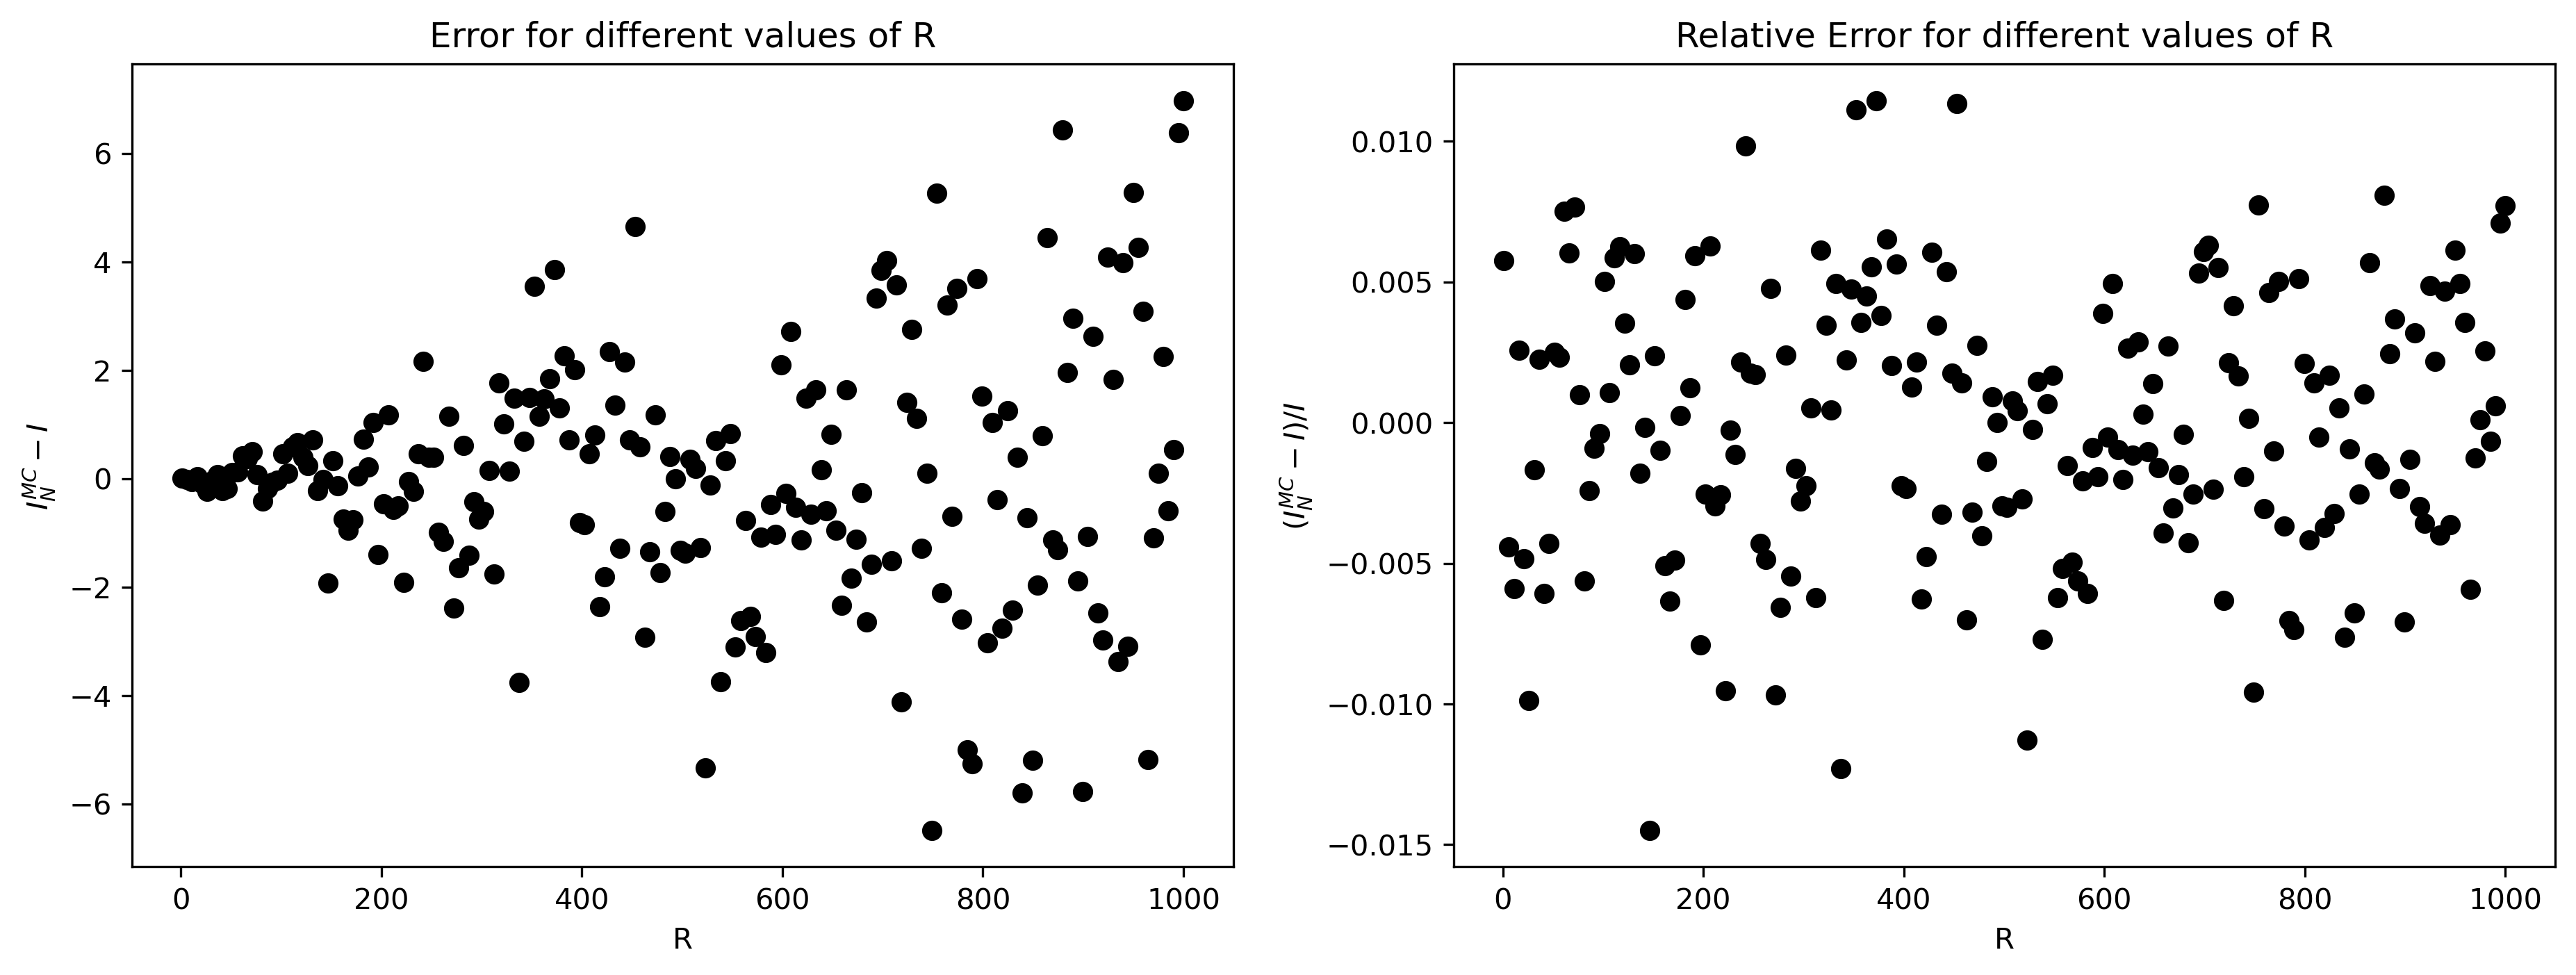
\includegraphics[width=\textwidth]{figure_simulation_R.png}
    \caption{Point estimates error and relative error for different values of $R$.}
    \label{fig:simulations-r}
\end{figure}

\end{proof}

\end{enumerate}



% 
\bibliographystyle{apalike}
\bibliography{../stat_comp}

\end{document}          